%(BEGIN_QUESTION)
% Copyright 2011, Tony R. Kuphaldt, released under the Creative Commons Attribution License (v 1.0)
% This means you may do almost anything with this work of mine, so long as you give me proper credit

Biomass gasification is a process where organic matter liberates flammable gases such as hydrogen (H$_{2}$) and carbon monoxide (CO) when heated to high temperatures.  A {\it gasifier} is a machine designed to heat the organic matter to the necessary temperature (usually by partial combustion) in order for this to occur:

$$\includegraphics[width=15.5cm]{i01535x01.eps}$$

Besides hydrogen and carbon monoxide, there are other gases mixed in the ``syngas'' outlet from the gasifier, which we desire to measure in order to properly control the chemical reactions happening inside the gasifier.  These include nitrogen oxide (NO) and carbon dioxide (CO$_{2}$).  Upon investigation, you discover two different gas analyzer technologies capable of accurately measuring all these gases: one is an {\it NDIR} (Non-dispersive infra-red) analyzer with multiple detectors, and the other is a {\it chromatograph}.  For this application, you happen to find analyzers of both types at comparable cost, which eliminates cost as a deciding factor when choosing the analyzer type.

NDIR analyzers typically have measurement dead times in the range of seconds, whereas chromatographs typically exhibit measurement dead times in the order of minutes.  Based on this criterion, which is the preferred analyzer technology for closed-loop control, and most importantly {\it why?}

\vskip 20pt \vbox{\hrule \hbox{\strut \vrule{} {\bf Suggestions for Socratic discussion} \vrule} \hrule}

\begin{itemize}
\item{} Explain why the differential pressure transmitter has its {\it low-pressure} port connected to the gasifier (with the high-pressure port vented), rather than the other way around.
\item{} Explain why a {\it VFD} is a good choice for a final control element on the syngas line, as opposed to a constant-speed blower and a control valve.  
\item{} Identify the most significant safety hazard(s) inherent to this process, as well as any PPE (Personal Protective Equipment) operators and technicians could use while working near it.
\end{itemize}

\underbar{file i01535}
%(END_QUESTION)





%(BEGIN_ANSWER)

The NDIR analyzer is clearly the better choice from the perspective of dead time.  More dead time in a feedback loop results in slower (possible) automatic control response, because a controller response appropriate for a minimal-deadtime loop will oscillate given the presence of additional dead time.

For a more complete explanation of this, refer to {\it Lessons In Industrial Instrumentation} in the section describing ``dead time'' as a process characteristic, and how its presence affects feedback control.

%(END_ANSWER)





%(BEGIN_NOTES)

The NDIR analyzer, having less dead time than a chromatograph, would be the better choice for closed-loop control.

\vfil \eject

\noindent
{\bf Summary Quiz:}

Explain why {\it dead time} is a bad thing to have in a feedback control loop.

\begin{itemize}
\item{} Dead time delays the controller's switching from auto to manual
\vskip 5pt 
\item{} Dead time makes oscillation (cycling) much more likely to occur
\vskip 5pt 
\item{} Dead time skews the accuracy of the control valve's positioning
\vskip 5pt 
\item{} Dead time skews the accuracy of the measurement under steady-state conditions
\vskip 5pt 
\item{} Dead time limits the maximum process production rate 
\vskip 5pt 
\item{} Dead time causes the control valve to travel more, prematurely wearing it out
\end{itemize}


%INDEX% Control, basics: process dead time
%INDEX% Measurement, analytical: chromatography
%INDEX% Measurement, analytical: nondispersive optical
%INDEX% Process: biomass gasification (downdraft gasifier)

%(END_NOTES)


